Maskinens alla delar ritas med användning av ”SolidWorks” som är ett CAD program. Utöver möjligheten att rita möjliggör SolidWorks simulering av de ritade delarna. Med denna egenskap kan man kontrollera och se hur maskinenes olika delar fungerar ihop som en maskin. På programmets simulator kan man påverka en visuell kraft på en del och avsyna hur den reagerar innan man konstruerar en del.
\begin{figure}[ht]
	\begin{center}
		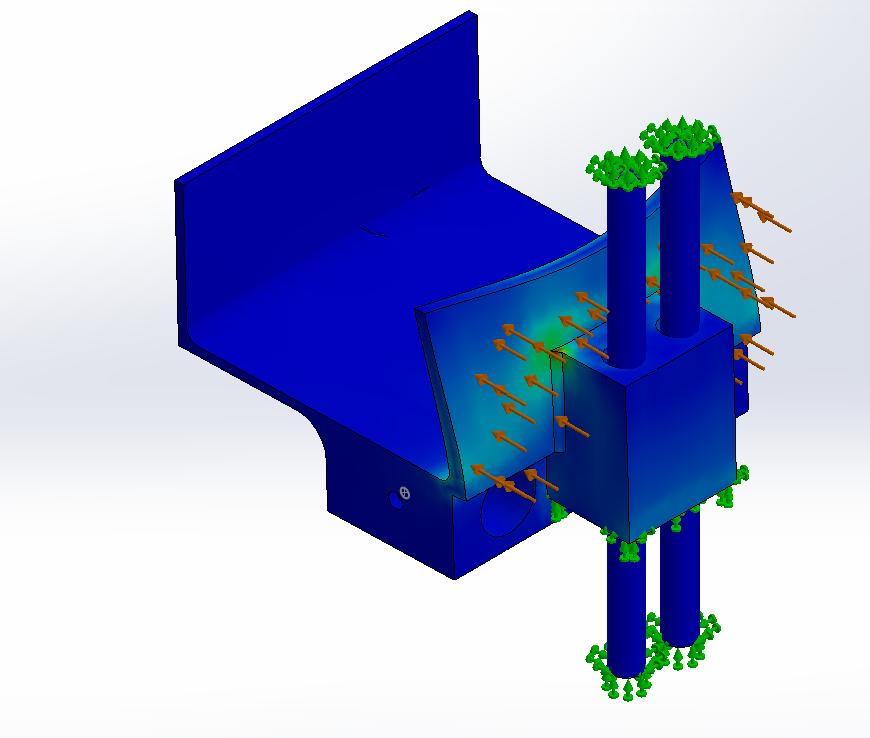
\includegraphics[scale=0.8]{images/hissEdited.png}
		\caption{Exempel på visuell kraf påverkat på en del i SolidWorks. Större spänning visas grönt.}
		\label{simulering}	
	\end{center}
\end{figure}